\documentclass[a4paper,11pt]{article}

% Identificação
\newcommand{\pbtitulo}{MongoDB com Java e Python}
\newcommand{\pbversao}{1.2}

\usepackage{../sty/tutorial}

%----------------------------------------------------------------------
% Início do Documento
%----------------------------------------------------------------------
\begin{document}
	
\maketitle % mostrar o título
\thispagestyle{fancy} % habilitar o cabeçalho/rodapé das páginas

%----------------------------------------------------------------------
% RESUMO DO ARTIGO
%----------------------------------------------------------------------
	
\begin{abstract}
	\initial{A}\textbf{tualmente muito se tem comentado sobre bancos de dados não relacionais, também chamados de NoSQL. O conhecimento destes podem abrir várias portas e deve ser considerado um fator de extrema importância para garantir uma boa empregabilidade. É sempre importante estar atento a novas tecnologias e como elas resolvem problemas provenientes das limitações existentes no caso deste tipo de banco enormes quantidade de dados. Neste tutorial veremos o que vem a ser o banco MongoDB \cite{mongooficial} e como proceder sua utilização utilizando como pano de fundo a linguagem de programação Java \cite{javaoficial} e Python \cite{pythonoficial}.}
\end{abstract}

%-----------------------------------------------------------------------------
% CONTEÚDO DO ARTIGO
%-----------------------------------------------------------------------------

\section{Parte inicial}
MongoDB (de ``humongous'' - monstruoso) é um Sistema de Banco de dados não relacional, Orientado a Documentos e de fonte aberto. É parte da família de sistemas de Banco de Dados denominados \textbf{NoSQL}, ou seja, em vez de armazenar dados em tabelas - como é feito em um banco de dados relacional - armazena seus dados em uma estrutura como JSON, ou seja, documentos com esquemas dinâmicos. Este formato é conhecido como \textbf{JSON Binário} ou simplesmente BSON.
\begin{figure}[H]
	\centering
	
\includegraphics[width=0.5\textwidth]{imagens/logo.jpg}
	\caption{Logo do MongoDB}
\end{figure}

Possui como objetivo principal promover uma integração mais fácil e rápida com os dados. E possui as seguintes características:
\begin{itemize}[nolistsep]
  \item Escrito em linguagem de programação C++
  \item Gerenciar coleções de documentos BSON formato de intercâmbio de dados usado principalmente como um formato de armazenamento de dados e transferência de rede no banco de dados MongoDB.
  \item BSON é uma forma binária para a representação de estruturas de dados simples e matrizes associativas (chamados de objetos ou documentos no MongoDB)
\end{itemize}

\subsection{Criar o contêiner Docker}
A forma mais simples de termos o MongoDB é através de um contêiner no Docker, assim facilmente podemos ter várias versões do banco instalada e controlar mais facilmente qual banco está ativo ou não. E ainda colhemos o benefício adicional de não termos absolutamente nada deixando sujeira em nosso sistema operacional ou áreas de memória.

Baixar a imagem oficial: \\
\codigo{\$ docker pull mongo}

Criar uma instância do banco em um contêiner: \\
\codigo{\$ docker run --name meu-mongo -p 27017:27017 -d mongo}

Acessar o Shell de comandos do MongoDB no contêiner: \\
\codigo{\$ docker exec -it meu-mongo mongo admin}
\begin{lstlisting}[]
> show dbs
> use local
> show collections
> exit
\end{lstlisting}

Para encerrar o contêiner: \\
\codigo{\$ docker stop meu-mongo} 

Para iniciar novamente o contêiner: \\
\codigo{\$ docker start meu-mongo} 

\subsection{Shell - a console de comandos}
O Mongo Shell, também conhecida como Console de Comandos, utiliza uma interatividade entre comandos JavaScript e o MongoDB. Aqui é possível realizar operações administrativas como consultas ou manutenções de dados.

Mostrar as bases de dados existentes: \\
\codigo{> show dbs}

Criar (ou mudar) a base de dados para a atual: \\
\codigo{> use nome\_base}

Mostrar as coleções existentes na base de dados atual: \\
\codigo{> show collections}

* \textbf{db} deixar como está pois é uma variável interna que aponta para a base de dados atual e \textbf{col} deve ser modificada para o nome da coleção nas ações abaixo.

Inserir (ou alterar caso o objeto tenha sido chamado anteriormente) um documento em uma coleção (se a coleção não existe será criada) na base de dados corrente: \\
\codigo{> db.col.save(\{"campo1":"valor1", ..., "campoN":"valorN"\})} 

Listar os documentos de uma coleção existente na base de dados atual: \\
\codigo{> db.col.find()}

Listar um documento específico de uma coleção existente na base de dados atual: \\
\codigo{> db.col.find(\{"campo":"valor"\})}

Adicionar uma nova coluna: \\
\codigo{> db.col.update(\{\}, \{"\$set":\{"campo":"valor"\}\}, \{upsert:false, multi:false\})}

Eliminar documento(s) de uma coleção existente na base de dados atual: \\
\codigo{> db.col.remove(\{campo:valor\})}

Apagar uma coleção existente na base de dados atual: \\
\codigo{> db.col.drop()}

Apagar a base de dados atual: \\
\codigo{> db.dropDatabase()}

Se percebemos bem a única diferença do MongoDB para bancos relacionais é entendermos como é o relacionamento entre os objetos:
\begin{figure}[H]
	\centering
	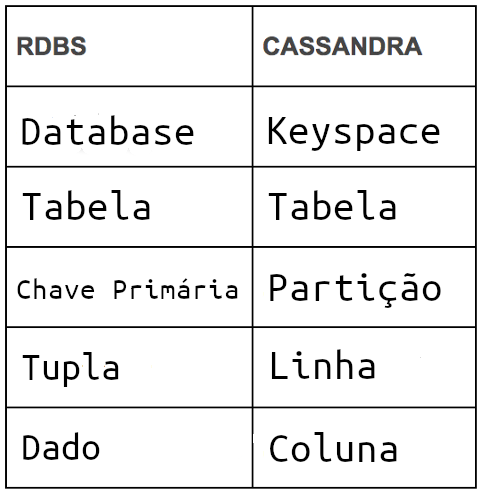
\includegraphics[width=0.5\textwidth]{imagens/comparativo.png}
	\caption{Comparativo entre os objetos do MongoDB e SQL}
\end{figure}

Para conhecer mais comandos do Shell, podemos acessar o seguinte endereço: \url{https://docs.mongodb.org/manual/mongo/}.
\section{Linguagem Java}
Java é considerada a linguagem de programação orientada a objetos mais utilizada no Mundo, base para a construção de ferramentas como Hadoop, Pentaho, Weka e muitas outras utilizadas comercialmente. Foi desenvolvida na década de 90 por uma equipe de programadores chefiada por \textit{James Gosling} para o projeto Green, na Sun Microsystems - tornou-se nessa época como a linguagem que os programadores mais baixaram e o sucesso foi instantâneo. Em 2008 o Java foi adquirido pela Oracle Corporation.

\subsection{Driver JDBC de Conexão}
Para proceder a conexão com Java, é necessário baixar um driver JDBC (Java Database Connection). Existem vários drivers construídos. Para utilizar o driver é necessário criar um projeto (vamos usar o \textbf{Spring Tool Suite 4}, utilize se quiser qualquer outro editor de sua preferência).

No STS4 acessar a seguinte opção no menu: File $\triangleright$ New $\triangleright$ Java Project. Informar o nome do projeto (Decus), não esquecer de modificar a opção "Use an environment JRE" para a versão correta da Java Runtime desejada e pressionar o botão Finish.

Agora devemos convertê-lo para um projeto Apache Maven. Clicar com o botão direito do mouse no projeto e acessar a opção: Configure $\triangleright$ Convert to Maven Project. Na janela apenas pressione o botão \textit{Finish}. Se tudo está correto observamos que o projeto ganhou uma letra \textbf{M} o que indica agora é um projeto padrão Maven. Então foi criado um arquivo chamado \textbf{pom.xml}. 

Acessar este arquivo e antes da tag BUILD, inserir a tag DEPENDENCIES:
\begin{lstlisting}[]
<dependencies>
  <dependency>
    <groupId>redis.clients</groupId>
    <artifactId>jedis</artifactId>
    <version>2.8.1</version>
  </dependency>
</dependencies>
\end{lstlisting}

Agora a situação do projeto é esta:
\begin{figure}[H]
	\centering
	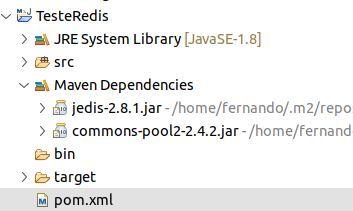
\includegraphics[width=0.5\textwidth]{imagens/dependenciasMaven}
	\caption{Dependências do Maven}
\end{figure}

Observamos que na pasta \textbf{Maven Dependencias} foi baixado a versão 2.8.1 do driver Jedis - Isso não é erro de digitação realmente o driver se escreve com "J".

\subsection{Exemplo Prático de uma Escola}
Estamos prontos para testarmos a conexão entre Redis e Java. Criamos um pequeno exemplo que nos auxiliará como teste, uma classe chamada \textbf{Escola} no pacote \textbf{decus.com} e inserimos nesta a seguinte codificação:
\begin{lstlisting}[]
package decus.com;

import java.text.SimpleDateFormat;
import java.util.Date;

import redis.clients.jedis.Jedis;

public class Escola {
	
	private String [] materias = new String[] {
	  "Matemática Computacional", "Programação", "Estatística",
  	  "SQL", "NoSQL", "Java", "Python", "Análise de Dados",
	  "Arquitetura de DW", "Big Data"
    };

	public static void main(String [] args) {
		new Escola().executar();
	}
	
	private void executar() {
		adicionarNotas();
	}
}
\end{lstlisting}

Nossa escola promove cursos mensais e temos um conjunto contendo todas as matérias que são aplicadas aos alunos. Ao término do curso é registrado o nome do aluno, a matéria e sua nota. Escolhemos o Redis para conter esses dados exatamente devido a sua característica de chave-valor.

No método principal que chama o executar, em Java não devemos programar no método "main". No executar colocamos uma chamada ao método criarAlunos() que terá a seguinte codificação:
\begin{lstlisting}[]
  private void adicionarNotas() {
	Jedis jedis = new Jedis();
	String data = new SimpleDateFormat("dd/MM/yyyy").format(new Date());
	String chave = "";
	String [] nomes = new String[] {
	  "Alice", "Miguel", "Sophia", "Arthur", "Helena", "Bernardo", "Valentina", 
	  "Heitor", "Laura", "Davi", "Isabella", "Lorenzo", "Manuela", "Théo", "Júlia", 
	  "Pedro", "Heloísa", "Gabriel", "Luiza", "Enzo", "Maria", "Luiza", "Matheus", 
	  "Lorena", "Lucas", "Lívia", "Benjamin", "Giovanna", "Nicolas", "Maria", 
	  "Eduarda", "Guilherme", "Beatriz", "Rafael", "Clara", "Joaquim", "Cecília"
	};
	String nome = "";
	for (int i = 0; i < 50; i++) {
	  nome = nomes[(int)(Math.random()*nomes.length)] + " " + nomes[(int)(Math.random()*nomes.length)];
  	  for (int j = 0; j < materias.length; j++) {
	    chave = "MAT" + i + "-" + j + "-" + data;
		jedis.hset(chave, "nome", nome);
		jedis.hset(chave, "materia", materias[j]);
		jedis.hset(chave, "nota", ""+(int)(Math.random()*11));
		jedis.close();
	  }
	}
	System.out.println("Notas Adicionadas");
  }
\end{lstlisting}

Obviamente como isto é um simples exemplo vamos adicionar as notas de uma forma totalmente aleatória.

Neste método temos a definição do objeto do Jedis que é responsável pela comunicação com o banco de dados que deve estar disponível na porta padrão. Criamos duas listas de nomes e matérias apenas para compor as notas que iremos inserir e ter dados mais elaborados. Teremos 50 alunos que ganharão nomes e sobrenomes completamente aleatórios com base na primeira lista, para cada um deles percorremos a lista de matéria e definimos uma chave que será composta por: "MAT" + valor de i (que é o número do aluno) + valor de j (que é o número da materia) e a data que estamos inserindo a informação. Assim temos a garantia que essa chave será única.

Para inserir a informação no objeto Jedis temos o método "hset" que recebe 3 parâmetros a chave, o nome do campo e o valor deste, e assim inserimos os campos nome, matéria e nota que será obtida também de forma aleatória (entre o valor de 0 a 10). Uma vez executado temos como resposta na console a mensagem "Notas Adicionadas" se verificamos no aplicativo "Another Redis Desktop Manager" teremos os seguintes dados:
\begin{figure}[H]
	\centering
	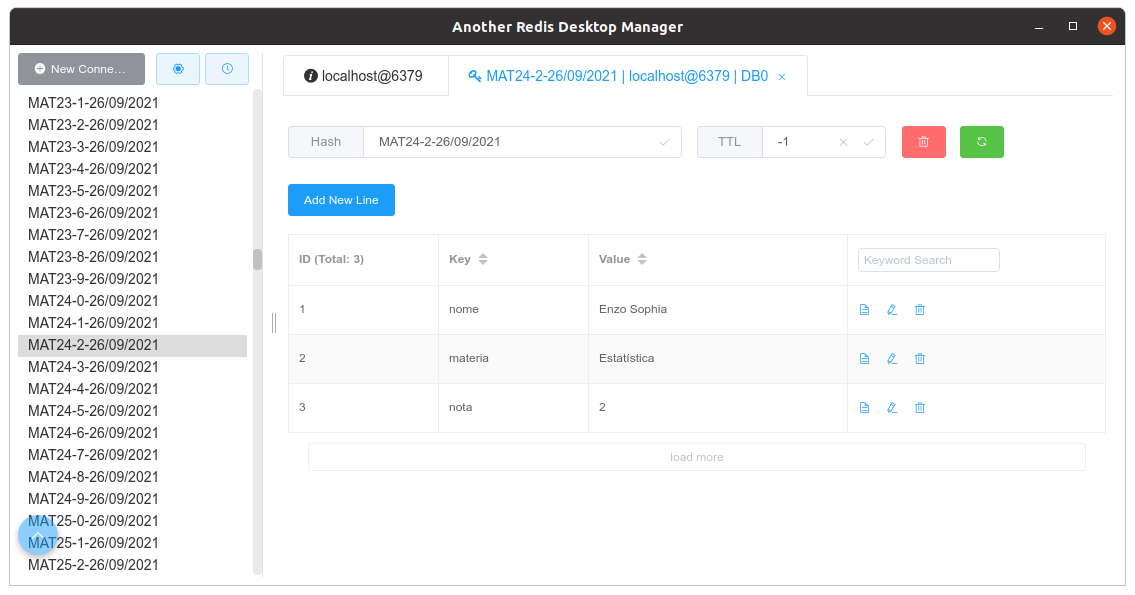
\includegraphics[width=0.8\textwidth]{imagens/notasAlunos}
	\caption{Another Redis Desktop Manager}
\end{figure}

Obviamente que os dados podem dar diferença pois o nome e as notas foram selecionados randomicamente.

\subsection{Localizações}
No método executar comentamos a chamada ao método "adicionarNotas()" e criamos outra para o método "trazerAluno(1)" que terá a seguinte codificação:
\begin{lstlisting}[]
  private void trazerAluno(int mat) {
	Jedis jedis = new Jedis();
	Set<String> nomes = jedis.keys("MAT" + mat + "-*");
	java.util.Iterator<String> it = nomes.iterator();
	String s;
	while (it.hasNext()) {
      s = it.next();
      System.out.print(jedis.hget(s, "nome") + " - ");
      System.out.print(jedis.hget(s, "materia") + " - ");
      System.out.println(jedis.hget(s, "nota"));
	}
	jedis.close();
  }	
\end{lstlisting}

As coisas no Redis são bem fáceis e rápidas, recebemos a matrícula e obtemos um conjunto (objeto Set) com todas as chaves que começam pela expressão "MAT1-" (como o valor que passamos foi 1) podemos utilizar esse método para realizar qualquer tipo de pesquisa, por exemplo "*-26/09/2021" trará todas as chaves do dia "26/09/2021". 

Percorremos esse conjunto e obtemos os dados que desejamos através do método "hget" no qual passamos a chave e o campo que desejamos. Ao executarmos teremos na console o nome do aluno, o nome da matéria e a nota obtida por esse.

Mas e se por exemplo desejamos saber a média geral das matérias dessa turma em cada matéria? Comentamos a chamada ao "trazerAluno(1)" no método executar por "mediaGeral()" e adicionamos a seguinte codificação:
\begin{lstlisting}[]
  private void mediaGeral() {
	Jedis jedis = new Jedis();
	String materia = "";
	for (int i = 0; i < materias.length; i++) { 
		int totNota = 0;
		int qtdNota = 0;
		Set<String> nomes = jedis.keys("*-"+i+"-*");
		java.util.Iterator<String> it = nomes.iterator();
		String s;
		while (it.hasNext()) {
			s = it.next();
			materia = jedis.hget(s, "materia");
			totNota += Integer.parseInt(jedis.hget(s, "nota"));
			qtdNota++;
		}
		System.out.println(materia + " - " + (totNota/qtdNota));
	}
	jedis.close();
  }	
\end{lstlisting}

E temos na saída da console cada uma das matérias e sua respectiva média.

\subsection{Eliminar Registro}
Assim como a consulta do registro é obtida através da chave o mesmo se aplica para a eliminação do mesmo, vamos comentar a chamada ao método "mediaGeral()" e chamar o método "eliminarAluno(1)" e adicionarmos a seguinte  codificação:
\begin{lstlisting}[]
  private void eliminarAluno(int mat) {
	Jedis jedis = new Jedis();
	Set<String> nomes = jedis.keys("MAT" + mat + "-*");
	java.util.Iterator<String> it = nomes.iterator();
	String s;
	while (it.hasNext()) {
		s = it.next();
		jedis.del(s);
	}
	jedis.close();
	System.out.println("Notas Eliminadas");
  } 	
\end{lstlisting}

Localizamos as chaves do aluno e executamos o método "del(chave)" para cada registro. Ou seja, extremamente simples e prático.

\subsection{Estrutura do objeto Jedis}
Aqui utilizamos o modelo estrutural de um Hash com mapeamento de um campo String como no de campo e seu respectivo valor e que pode ser aplicado para a grande maioria dos casos, porém existem outras estruturas no Redis que podem ser utilizadas com este conector.

\textbf{String}

É o modelo mais simples uma chave e um valor, pode ser utilizado por exemplo para uma associação de palavras como localidade e endereço:
\begin{lstlisting}[]
  jedis.set("Joaquim Lucas", "Qd 28 Casa 47 Rua Amélia Cidade Vale Alegre");
  jedis.set("Nicolas Cecília", "Qd 7 Casa 7 Rua Sete da Cidade Amarela");
  
  System.out.println(jedis.get("Joaquim Lucas"));
\end{lstlisting}

Ou seja, utilizamos o método "set(chave, valor)" para inserirmos a informação e o método "get(chave)" para obtê-la. Esse modelo também pode ser utilizado como uma camada de cache extremamente rápida e simples de se usar para solicitações HTTP recebidas de um aplicativo Web ou outros requisitos de cache. 

\textbf{Listas}

São listas de strings, classificadas por ordem de inserção e podem ser uma ferramenta ideal para implementar, por exemplo, filas de mensagens:
\begin{lstlisting}[]
jedis.lpush("tarefas", "Primeira tarefa do dia");
jedis.lpush("tarefas", "Segunda tarefa do dia");
jedis.lpush("tarefas", "Terceira tarefa do dia");
\end{lstlisting}

A cada comando "lpush(chave, valor)" uma nova tarefa é inserida. Para retirar usamos o comando:
\begin{lstlisting}[]
System.out.println(jedis.rpop("tarefas"));
\end{lstlisting}

Devemos lembrar que precisamos serializar qualquer objeto e persisti-lo como uma string, portanto, as mensagens na fila podem transportar dados mais complexos quando necessário.

\textbf{Conjuntos}

Trata de uma coleção não ordenada de Strings e que são bem úteis quando desejamos excluir membros repetidos, para adicionar elementos usamos:
\begin{lstlisting}[]
jedis.sadd("frutas", "abacate");
jedis.sadd("frutas", "manga");
jedis.sadd("frutas", "abacate");

Set<String> conjunto = jedis.smembers("frutas");
System.out.println(jedis.sismember("frutas", "abacate"));
\end{lstlisting}

As frutas do Java Set terão um tamanho de 2, a segunda adição de "abacate" foi ignorada. O método sismember permite que verifiquemos a existência de um membro específico rapidamente e mesmo com a resposta "true" se olharmos no nosso banco (usemos o aplicativo "Another Redis Desktop Manager") veremos que só existe uma única ocorrência para "abacate".
\begin{figure}[H]
	\centering
	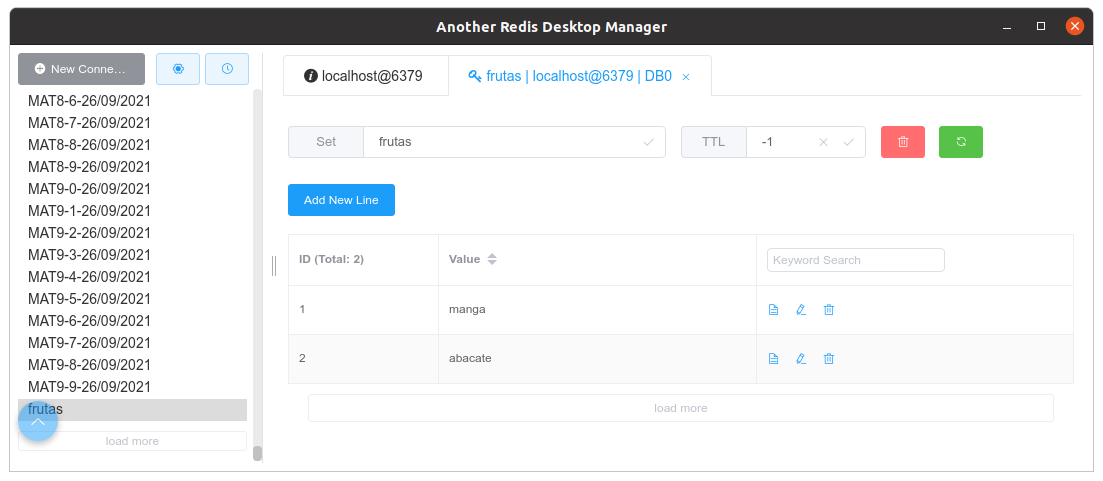
\includegraphics[width=0.8\textwidth]{imagens/frutas}
	\caption{Visão do Conjunto Frutas}
\end{figure}

\textbf{Conjuntos Ordenados}
São conjuntos classificados em que cada membro possui uma determinada classificação associada, que é usada para localizá-los. Podemos inserir alguns alunos e seus desempenhos da seguinte forma:
\begin{lstlisting}[]
Map<String, Double> desempenho = new HashMap<>();
desempenho.put("Aluno 1", 3000.0);
desempenho.put("Aluno 2", 1500.0);
desempenho.put("Aluno 3", 8200.0);
desempenho.put("Aluno 4", 2500.0);
desempenho.put("Aluno 5", 7500.0);
desempenho.put("Aluno 6", 6200.0);
desempenho.entrySet().forEach(playerScore -> {
  jedis.zadd("Desempenho", playerScore.getValue(), playerScore.getKey());
});	
\end{lstlisting}

E obtermos uma relação dos 3 melhores com a seguinte codificação:
\begin{lstlisting}[]
System.out.println("1o.: " + jedis.zrevrange("Desempenho", 0, 1).iterator().next());
System.out.println("2o.: " + jedis.zrevrange("Desempenho", 1, 2).iterator().next());
System.out.println("3o.: " + jedis.zrevrange("Desempenho", 2, 3).iterator().next());
\end{lstlisting}

Podemos utilizar de todas essas estruturas para criarmos uma aplicação extremamente veloz ou mesmo usar o Redis como um complementar para determinadas ações que precisamos aumentar os ganhos de velocidade.

\section{Python}
Python é uma linguagem de programação de alto nível, interpretada a partir de um script, Orientada a Objetos e de tipagem dinâmica. Foi lançada por Guido van Rossum em 1991. Não pretendo nesta apostila COMPARAR essa linguagem com Java (espero que nunca o faça), fica claro que os comandos são bem mais fáceis porém essas linguagens possuem diferentes propósitos.

Todos os comandos descritos abaixo foi utilizado no JupyterLab \cite{jupyteroficial}, então basta abrir um Notebook e digitá-los em cada célula conforme se apresentam.

\subsection{Proceder a Conexão}
Baixar o pacote necessário: \\
\codigo{ !pip install pymongo}

Importar os pacotes necessários: \\
\codigo{ from pymongo import MongoClient \\
	import random}

Neste caso estamos utilizando o pacote \textbf{random} somente para criarmos o mesmo exemplo já visto e escolher uma nota aleatória para casa aluno.

Nos conectamos ao servidor desta forma: \\
\codigo{ cliente = MongoClient('localhost', 27017)}
Ou: \\
\codigo{ cliente = MongoClient('mongodb://localhost:27017/')}

Listar as bases disponíveis: \\
\codigo{ cliente.list\_database\_names()) }

Nos conectamos a uma base desta forma: \\
\codigo{ db = cliente.escola}
Ou: \\
\codigo{ db = cliente['escola']}

Listar as coleções disponíveis: \\
\codigo{ cliente.list\_collection\_names()) }

Nos conectamos a uma coleção desta forma: \\
\codigo{ col = db.aluno}
Ou: \\
\codigo{ col = db['aluno']}

\subsection{Inserir documentos}
Inserir um único documento é uma questão de criar um dicionário e enviá-lo para a coleção: \\
\codigo{ mario = \{ "nome": "Mario da Silva", "nota": random.randint(1,11) \} \\
	col.insert\_one(mario) }

Inserir vários documentos é necessário criar uma lista de dicionários e enviar a lista para a coleção: \\
\codigo{ alunos = [ \\
	\phantom{x}\hspace{4pt} \{ "nome": "Aline Moraes", "nota": random.randint(1,11) \}, \\
	\phantom{x}\hspace{4pt} \{ "nome": "Soraya Gomes", "nota": random.randint(1,11) \} \\
	] \\
	col.insert\_many(alunos)
}

\subsection{Encontrar documentos}
Listar toda a coleção: \\
\codigo{ for doc in col.find(\{\}): \\
	\phantom{x}\hspace{4pt} print(doc)}

Listar toda a coleção de modo ordenado ascendente (ou descendente - valor -1): \\
\codigo{for doc in col.find(\{\}).sort("campo",1): \\
	\phantom{x}\hspace{4pt} print(doc)}

Quantos documentos existem na coleção: \\
\codigo{ col.count\_documents(\{\})}

Trazer o primeiro documento: \\
\codigo{ col.find\_one()}

Trazer um determinado documento: \\
\codigo{ col.find\_one(\{"nome": "Aline Moraes"\})}

Limitar a quantidade de documentos buscados (no caso 5): \\
\codigo{for doc in col.find(\{\}).limit(5): \\
	\phantom{x}\hspace{4pt} print(doc)}

Mostrar um determinado campo (e somente ele): \\
\codigo{for doc in col.find(\{\}): \\
	\phantom{x}\hspace{4pt} print(doc['col'])}

Trazer os documentos que possuem a nota maior que 5 e menor que 7: \\
\codigo{ for doc in col.find(\{"nota": \{"\$gt": 5, "\$lt": 7\}\}): \\
	\phantom{x}\hspace{4pt} print(doc)}

\subsection{Atualizar documentos}
* O lado da esquerda é o filtro de consulta e o lado do SET são os campos a alterar.

Alterar um documento que possui o nome "Mario da Silva": \\
\codigo{ col.update\_one(\{"nome": "Mario da Silva"\}, \{"\$set": \{"nota": 8\}\})}

Alterar os documentos que possuem a nota menor que 5: \\
\codigo{ col.update\_many(\{'nota': \{'\$lt': 5\}\}, \{'\$set': \{'nota': 4\}\})}

Eliminar um documento que possui o nome "Mario da Silva": \\
\codigo{ col.delete\_one(\{"nome": "Mario da Silva"\})}

Eliminar os documentos que possuem a nota menor que 5: \\
\codigo{ col.delete\_many(\{'nota': \{'\$lt': 5\}\})}

\subsection{Encerrar}
É boa prática fechar a base de dados: \\
\codigo{ cliente.close()}

Mas antes de encerramos realmente vejamos o seguinte programa completo em linguagem Python:

\begin{lstlisting}[]
from pymongo import MongoClient
from random import randint

# Passo 1: Conectar ao Mongo
cliente = MongoClient(port=27017)
db = cliente.negocio

# Passo 2: Criar Amostras de Dados
nomes = ['Kitchen', 'Espiritual', 'Mongo', 'Tastey', 'Big', 'Jr', 'Filho', 'City', 'Linux'
         'Tubarão', 'Gado', 'Sagrado', 'Solo', 'Sumo', 'Lazy', 'Fun', 'Prazer', 'Gula']
tipo_emp = ['LLC', 'Inc', 'Cia', 'Corp.']
tipo_coz = ['Pizza', 'Bar', 'Fast Food', 'Italiana', 'Mexicana',
            'Americana', 'Sushi', 'Vegetariana', 'Churrascaria']

for x in range(1, 501):
  nome1 = nomes[randint(0, (len(nomes)-1))]
  nome2 = nomes[randint(0, (len(nomes)-1))]
  tipoE = tipo_emp[randint(0, (len(tipo_emp)-1))]
  negocio = {
	'nome': nome1 + ' ' + nome2 + ' ' + tipoE,
	'nota': randint(1, 5),
	'cozinha': tipo_coz[randint(0, (len(tipo_coz)-1))]
  }  

# Passo 3: Inserir o objeto negócio no banco
result = db.restaurante.insert_one(negocio)

# Passo 4: Mostrar no console o Object ID do Documento
print('Criado {0} de 500 como {1}'.format(x, result.inserted_id))

# Passo 5: Mostrar mensagem final
print('500 Novos Negócios Culinários foram criados...')
cliente.close()
\end{lstlisting}

O programa está auto-documentado e criar uma base com 500 registros.

\section{Conclusão}
Penso que depois dessa apostila, será possível usar todo o poder do banco MongoDB para seus trabalhos, pois como vimos é bem fácil realizar os passos nesse banco pouco importa a linguagem de programação. Não busquei nesta mostrar um exemplo mais completo para não limitar suas pesquisas e devemos considerar esta apenas como um pontapé inicial (\textit{KickStart}) para seus projetos.

Como visto o banco de dados MongoDB pode ser facilmente utilizado com aplicações em linguagem Java ou gerar os modelos para \textit{Machine Learning} com Python e ainda colher o benefício de substituir os bancos de dados relacionais para grandes quantidades de dados, sendo que esta é a grande motivação para NoSQL como forma de resolver o problema de escalabilidade dos bancos tradicionais.

Sou um entusiasta do mundo \textbf{Open Source} e novas tecnologias. Qual a diferença entre Livre e Open Source? \underline{Livre} significa que esta apostila é gratuita e pode ser compartilhada a vontade. \underline{Open Source} além de livre todos os arquivos que permitem a geração desta (chamados de arquivos fontes) devem ser disponibilizados para que qualquer pessoa possa modificar ao seu prazer, gerar novas, complementar ou fazer o que quiser. Os fontes da apostila (que foi produzida com o LaTex) está disponibilizado no GitHub \cite{github}. Veja ainda outros artigos que publico sobre tecnologia através do meu Blog Oficial \cite{fernandoanselmo}.

%-----------------------------------------------------------------------------
% REFERÊNCIAS
%-----------------------------------------------------------------------------
\begin{thebibliography}{8}
  \bibitem{mongooficial} 
  Página do Banco MongoDB \\
  \url{https://www.mongodb.org/}

  \bibitem{javaoficial} 
  Página do Oracle Java \\
  \url{http://www.oracle.com/technetwork/java/}
  
  \bibitem{pythonoficial} 
  Página do Python \\
  \url{https://www.python.org/}

  \bibitem{sts} 
  Editor Spring Tool Suite para códigos Java \\
  \url{https://spring.io/tools}

  \bibitem{jupyteroficial} 
  Página do Jupyter \\
  \url{https://jupyter.org/}

  	\bibitem{fernandoanselmo} 
	Fernando Anselmo - Blog Oficial de Tecnologia \\
	\url{http://www.fernandoanselmo.blogspot.com.br/}
	
	\bibitem{publicacao} 
	Encontre essa e outras publicações em \\
	\url{https://cetrex.academia.edu/FernandoAnselmo}
	
	\bibitem{github} 
	Repositório para os fontes da apostila \\
	\url{https://github.com/fernandoans/publicacoes}
\end{thebibliography}
  
\end{document}
